\documentclass[11pt]{abntex2}
\usepackage[utf8]{inputenc}
\usepackage[brazil]{babel}
\usepackage{indentfirst}
\usepackage{graphicx}
\usepackage{float}
\usepackage{enumitem}
\usepackage{mathtools}
\usepackage{pdflscape}
\usepackage{textcomp}
\usepackage[num, overcite]{abntex2cite}
\citebrackets[]
    
\titulo{Módulo remoto para ensaios de vibração}
\autor{Francisco Gomes Soares Sanches Manso}
\data{\today}
\instituicao{%
Universidade Federal de Minas Gerais - UFMG
\par
Escola de Engenharia
\par
Kotchergenko Engenharia Ltda.}
\local{Belo Horizonte}
\preambulo{Monografia apresentada durante o Seminário dos Trabalhos de Conclusão do Curso de Graduação em
Engenharia Elétrica da UFMG, como parte dos requisitos necessários à obtenção do título de Engenheiro Eletricista}
\orientador[Orientador:]{Ricardo de Oliveira Duarte}
\coorientador[Supervisor:]{Bruno Freitas Brant}

\begin{document}
\makeatletter
	\imprimircapa
	\imprimirfolhaderosto

	\begin{resumo}
		
	\end{resumo}

	\tableofcontents
	\newpage
	\listoffigures
	\newpage
	
	\chapter{Introdução}
		A mineração no Brasil possui grande importância na economia atual do país e
		do mundo e é um dos setores em maior expansão. Atividades nessa área já
		representam em torno de 5\% do PIB do país e geram mais de dois milhões de
		empregos diretos e indiretos.\cite{pib}

		Novas tecnologias vêm alavancando esse setor, buscando aumentar a eficiência
		de produção e transporte e o aproveitamento de resíduos para a
		transformação em insumos. A Escola de Engenharia da Universidade Federal de
		Minas Gerais (UFMG), por exemplo, desenvolve metodologias de calcificação
		dos resíduos da mineração, os tornando matéria-prima para a fabricação de
		produtos das áreas de construção civil. Esse reaproveitamento chega a
		proporcionar uma redução de até 40\% no custo das obras.\cite{mineracaoUFMG}
		
		O setor de mineração conta com diversas estruturas de grande porte em
		terminais portuários e ferrovias por todo o Brasil. A manutenção
		preditiva e o diagnóstico de falha são duas atividades de extrema
		importância no âmbito de possibilitar a segurança dos operadores, a
		redução de custos em bloqueios de produção por falhas e uma melhor
		modelagem da dinâmicas das estruturas utilizadas. Nesse sentido,
		diversas empresas da área baseiam suas atividades em três grandes
		pilares: a metodologia teórica de análise de estruturas, a capacidade de
		modelagem e simulação via \textit{software} e um preciso e confiável
		ensaio de campo para a obtenção de dados.
		
		Ensaios de campo de vibração e extensometria são comumente realizados
		utilizando equipamentos capazes de fazer aquisição de dados em tempo
		real de vários canais simultaneamente. Os ensaios de vibração, por
		exemplo, utilizam sensores piezoelétricos uniaxiais que são ligados em
		sistemas de aquisição, como o NI-9234 da National
		Instruments\textsuperscript{TM}.
		
		Os dados de vibração são obtidos por meio de sensores piezoelétricos com
		eletrônica integrada, conhecidos como sensores IEPE ou \textit{Integrated
		Electronics Piezo-Electric}. Materiais piezoelétricos são cristais capazes de
		gerar uma tensão elétrica após os aplicar uma força mecânica.
		Os transdutores IEPE pré-amplificam esse sinal de forma a possibilitar a
		condução dos mesmos através de cabos coaxiais.

		Tais ensaios são realizados em peneiras vibratórias de mineração,
        transportadores de correia e outras máquinas de áreas portuárias e ferroviárias.

		\chapter{Revisão Bibliográfica}
			No processo de amostragem de um sinal qualquer, deve-se filtrar o sinal com
			um filtro anti-\textit{aliasing} e aplicar os ganhos necessários para adequar
			o sinal à faixa de leitura do conversor analógico-digital. Os processos são
			ilustrados abaixo.

			\begin{figure}[H]
				\centering
				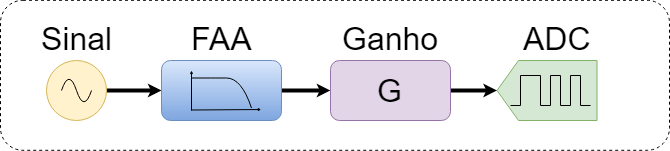
\includegraphics[width=\linewidth]{../../Fotos/Diagramas/sinalFaaADC/sinalFaaADC.png}
				\caption{Condicionamento do sinal analógico}
			\end{figure}

			A seguir, serão descritos cada parte que compõe este processo.

			\section{Transdutores piezoelétricos}
				Transdutores piezoelétricos são largamente utilizados para
				monitoramento industrial. Estes transdutores possuem uma eletrônica
				integrada que pré-amplifica e condiciona o sinal para melhor
				desempenho da medição. Os transdutores piezoelétricos com eletrônica
				integrada são denominados IEPE (\textit{Integrated Electronics
				Piezo-Electric}). Entre os transdutores, ou medidores, do tipo IEPE
				mais comuns, encontram-se os transdutores de pressão e de
				aceleração.

				Os medidores IEPE possuem variadas fichas técnicas, com diferentes
				faixas de alimentação, faixas de sinal de saída e tipos de sinal de
				saída. No caso dos medidores de aceleração com saída em tensão, os
				terminais de alimentação e de sinal de saída são compartilhados.

				Os transdutores de aceleração necessitam ser alimentados por uma
				tensão entre $18V$ e $30V$ com uma corrente constante de polarização
				entre $2ma$ e $10ma$, podendo variar de medidor para medidor. Para
				isso, utiliza-se uma fonte de tensão em série com uma fonte de
				corrente. Assim, o sinal de saída é a tensão imediatamente após a
				fonte de corrente. O esquemático abaixo ilustra o circuito elétrico
				equivalente da alimentação de um transdutor IEPE com saída em
				tensão.

				A conversão do sinal de saída para a grandeza de interesse é dada
				por uma relação linear de tensão e da unidade da grandeza. Essa
				relação é denominada sensibilidade. Como exemplo, toma-se o
				transdutor IEPE AC102, que possui sensibilidade de $100mV/g$.
				Assim, com um valor de fundo de escala de $\pm50g$, têm-se variações
				no valor da tensão de saída de $\pm5V$.\cite{ctc}
				\newpage

				\begin{figure}[H]
					\centering
					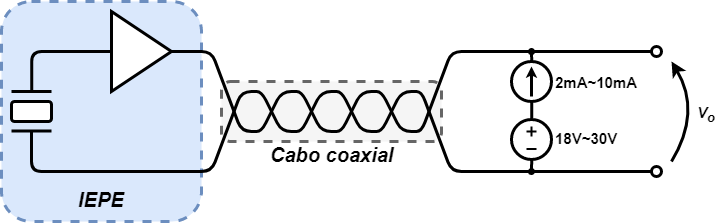
\includegraphics[width=\linewidth]{../../Fotos/Diagramas/iepe.png}
					\caption{Diagrama de interligação de um transdutor \textit{IEPE}}
				\end{figure}

			\section{O filtro anti-\textit{aliasing} e o teorema da amostragem}
				Seja um sinal $S(t)$ com maior componente de frequência
				$f_{max}$. Segundo o Teorema da Amostragem, ou Teorema de
				\textit{Nyquist}, esse sinal deve ser amostrado com uma
				frequência $f_s$ tal que $f_s>2f_{max}$. Caso contrário, o
				espectro de frequência irá sobrepor-se, impossibilitando a
				reconstrução correta do sinal no tempo. Esse fenômeno é denominado
				de \textit{aliasing} e a frequência $2\*f_{max}$ é definida como
				frequência de \textit{Nyquist}. \cite{nyquist}

				Como exemplo, assume-se o sinal $S(t) = 0,7\*sen(2\*\pi\*50\*t)
				+ sen(2\*\pi\*120\*t)$. O sinal é amostrado com uma frequência
				$f_s = 250Hz$. Os gráficos do sinal original, do sinal
				amostrado e da FFT (\textit{Fast Fourier Transform}), gerada a
				partir da aquisição do sinal na dada frequência de amostragem,
				são exibidos na Figura 3 e foram gerados através do
				\textit{software} Scilab

				Como a maior componente de frequência do sinal $S(t)$ é $120Hz$,
				a frequência de \textit{Nyquist} é $240Hz$. Assim, a taxa de
				amostragem satisfaz o Teorema da Amostragem. Com isso possibilita-se
				uma correta visualização da FFT e da reconstrução do sinal no tempo.

				Ao fazer uma segunda aquisição do mesmo sinal com uma taxa de
				amostragem $f_s = 200Hz$, obtém-se os gráficos exibidos na
				Figura 4. Como a frequência de amostragem é menor que a
				frequência de \textit{Nyquist} para este sinal, ocorre
				\textit{aliasing} e o sinal não é reconstruído corretamente.
				Esse erro também pode ser visto pela FFT, que apresenta
				frequências diferentes do sinal original.

				\newpage

				\begin{figure}[!ht]
					\centering
					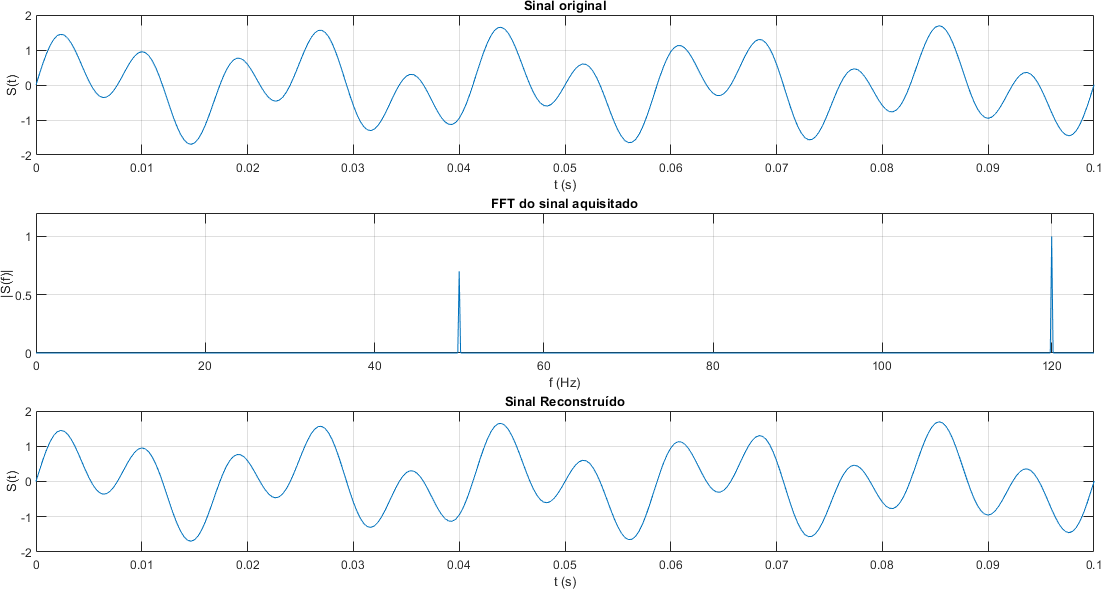
\includegraphics[width=\linewidth]{../../Fotos/aliasingFs250.png}
					\caption{Exemplo de sinal sem \textit{aliasing} amostrado à $250Hz$}
				\end{figure}

				\begin{figure}[H]
					\centering
					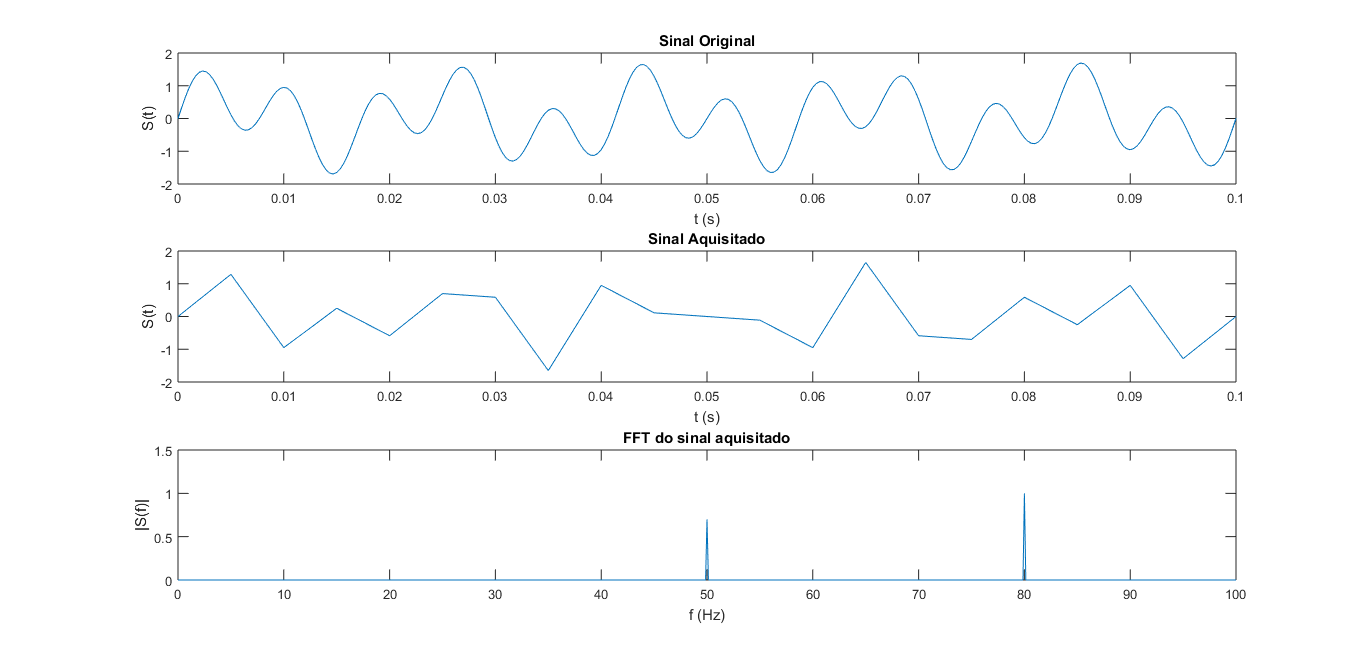
\includegraphics[width=\linewidth]{../../Fotos/aliasingFs200.png}
					\caption{Exemplo de sinal com \textit{aliasing} amostrado à $200Hz$}
				\end{figure}

				\pagebreak


				O filtro anti-\textit{aliasing} trata-se de um filtro passa-faixa
				ou passa-baixa. Como no projeto não há restrições com relação à
				baixas frequências, o filtro anti-\textit{aliasing} deste projeto
				é um filtro passa-baixa. Um filtro passa-baixa ideal possui
				característica de módulo em frequência mostrada na Figura 5.

				\begin{figure}[!ht]
					\centering
					\begin{minipage}{.4\linewidth}
						\centering
						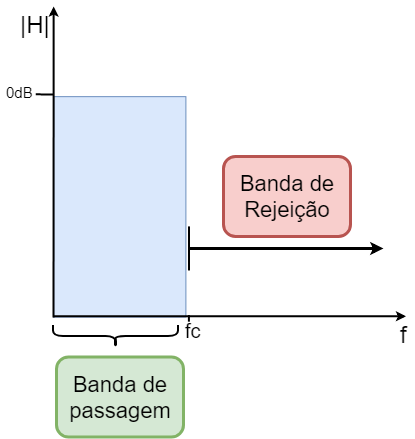
\includegraphics[width=.8\linewidth]{../../Fotos/Diagramas/sinalFaaADC/filtroIdeal.png}
						\caption{Resposta em frequência de um filtro ideal}
					\end{minipage}
					\hfill\vline\hfill
					\begin{minipage}{.4\linewidth}
						\centering
						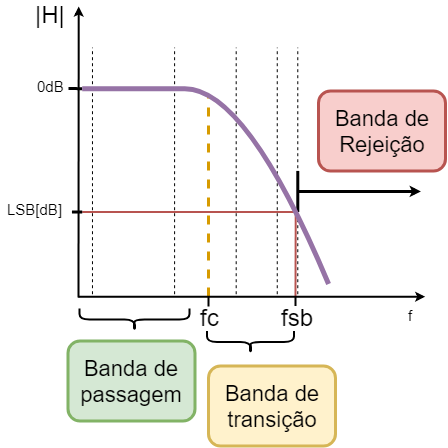
\includegraphics[width=\linewidth]{../../Fotos/Diagramas/sinalFaaADC/filtroReal.png}
						\caption{Resposta em frequência de um filtro real}
					\end{minipage}
				\end{figure}

				Entretanto, os filtros passa-baixa reais possuem uma banda a
				mais: a banda de transição. Essa banda representa os sinais de
				frequência cujas amplitudes não foram atenuadas suficientemente,
				de forma que não possam ser lidas pelo Conversor Analógico-Digital
				(ADC). Assim, se forem desprezadas na admissão da taxa de amostragem,
				podem gerar \textit{aliasing}.

				Com isso, em uma primeira análise, pode-se dizer que a frequência de
				amostragem deve satisfazer $f_s>2*f_{sb}$, em que $f_{sb}$ é chamada
				\textit{stop band frequency}, ou frequência da banda de rejeição.

				Não existe método capaz de reverter o \textit{aliasing} após o
				sinal ser amostrado. Então, o que deve ser feito é assumir uma
				faixa de frequência de interesse e utilizar circuitos capazes de
				atenuar frequências acima da frequência de \textit{Nyquist}.
				Essa atenuação deve ser tal que o ADC não possua resolução capaz
				de detectar as componentes de alta frequência. Os circuitos
				responsáveis por garantir que não ocorra \textit{aliasing} são
				denominados filtro anti-\textit{aliasing} (FAA).

			\section{Conversor analógico-digital}
				O conversor analógico-digital, ou ADC, é responsável por digitalizar
				um sinal analógico. A conversão é referenciada às tensões de alimentação
				do ADC e graduada de acordo com o número de \textit{bits}. Como exemplo,
				um conversor alimentado por uma tensão de $5V$ e com $10$ \textit{bits} de
				resolução possui $2^{10}$ divisões. Assim, a menor divisão do conversor é
				de $5/2^{10} = 4,88mV$ e, consequentemente, este é o menor valor que pode
				ser detectado pelo ADC. Se a resolução fosse de $12$ \textit{bits} ao invés
				de $10$ \textit{bits}, a resolução do conversor seria de $5/2^{12}=1,22mV$.
				Este também é o passo do conversor, também definido como LSB
				(\textit{Least Significant Bit}), ou seja, todas os valores digitalizados
				são múltiplos da resolução.

        \bibliography{../../Bibliografia/bibliografia}

\end{document}